\documentclass[a4paper,11pt]{article}
\usepackage[utf8]{inputenc}
\usepackage[T1]{fontenc}
\usepackage{graphicx}
\usepackage{amsmath}
\usepackage{geometry}
\geometry{margin=2.5cm}

\title{Documentazione della Pipeline Tabellare \\ \texttt{xai\_tab}}

\begin{document}
\maketitle

\section*{1. Contesto}
Per analizzare il fenomeno del \emph{Disagreement Problem} è stato scelto il dataset \emph{Breast–Cancer Wisconsin}, un dataset tabellare di 569 campioni e 30 caratteristiche numeriche, e due modelli MLP identici nell'architettura ma differenziati solo da diversi \emph{seed} di inizializzazione. 
L'obiettivo è capire quanto le mappe di importanza delle feature, generate con \emph{Integrated Gradients}, divergano tra i due modelli.

\section*{2. Tecnologie e librerie}
La pipeline è stata implementata in \textbf{Python 3.10} all'interno di un ambiente \texttt{conda} (\texttt{xai}) con:
\begin{itemize}
\item \textbf {PyTorch} per la definizione e il caricamento delle reti MLP;
\item \textbf {scikit-learn} per il preprocessing dei dati (standardizzazione e divisione in train/test);
\item Libreria \textbf {Captum} per la generazione delle spiegazioni \emph{Integrated Gradients};
\item \textbf {NumPy} per la gestione dei calcoli numerici su matrici;
\item \textbf {Matplotlib} per produrre le visualizzazioni (grafici a barre).
\end{itemize} 

\section*{3. Flusso di lavoro}
Il processo si articola in tre fasi: training dei modelli, generazione delle spiegazioni, calcolo delle metriche di disaccordo.

\subsection*{3.1 Training dei modelli (\texttt{train.py})}
Per prima cosa è stato caricato il dataset con \texttt{load\_breast\_cancer()}, applicato una standardizzazione (ogni feature riportata a media zero e varianza uno) e suddiviso i dati in training e test con split 80\%/20\%, mantenendo stabile la proporzione delle classi tramite \texttt{stratify=y} e fissando la riproducibilità con \texttt{random\_state=0}. 
Poi è stato definito una rete MLP a due layer nascosti da 16 neuroni ciascuno ed è stato ripetuto l’addestramento due volte, modificando soltanto il seed (0 e 1) per generare due modelli leggermente differenti pur mantenendo la stessa struttura. 
Ognuno di questi modelli è quindi salvato nei file \texttt{models/mlp\_seed0.pt} e \texttt{models/mlp\_seed1.pt}.

\subsection*{3.2 Generazione delle spiegazioni (\texttt{compare\_tabular.py})}
Nella fase successiva sono state caricate le feature di test, convertendole in tensori PyTorch (strutture dati multidimensionali che permettono di rappresentare un insieme di dati in maniera compatta ed efficiente), e importato i modelli precedentemente salvati, portandoli in modalità \texttt{eval()} per disattivare eventuali comportamenti di training come il dropout (processo di impostazione casuale di alcuni nodi a output zero durante il processo di addestramento). 

\paragraph{Baseline}
Per i metodi di attribution \emph{path‐integral} come Integrated Gradients, occorre un \emph{baseline}, ovvero un punto di riferimento da cui partire l’integrazione. In questo caso viene definito un vettore di zeri di dimensione pari al numero di feature (30):
\[
  \texttt{baseline} = \texttt{torch.zeros(1,30)}.
\]
Questa scelta equivale ad un campione “neutro” a cui tutte le feature contribuiscono per zero alla previsione.

\paragraph{Passi di integrazione (\texttt{n\_steps})}
Poiché l’Integrated Gradients calcola l’integrale del gradiente lungo il percorso dal \emph{baseline} al campione \(x\), tale integrale viene approssimato come somma di Riemann in \(m\) sotto‐intervalli. 
Ogni \emph{passo di integrazione} corrisponde al calcolo del gradiente in un punto intermedio:
\[
  x^{(k)} = x' + \frac{k}{m}\,(x - x'), 
  \quad k=1,\dots,m,
\]
dove \(x'\) è la baseline e \(m=\texttt{n\_steps}\). 
Maggiore è \(m\), più fedele è l’approssimazione e più “stabile” risulta la spiegazione, ma il costo computazionale cresce proporzionalmente. 
In questo caso è stato scelto \(m=50\).

\paragraph{Calcolo delle attributions}
Per ciascun modello si crea un oggetto \texttt{IntegratedGradients(model)} e si invoca:
\begin{verbatim}
attr = ig.attribute(X_test, baselines=baseline, n_steps=50)
\end{verbatim}
Il risultato è un tensore PyTorch di forma \((n\_samples,30)\), che poi convertiamo in NumPy (array unidimensionale) per le successive elaborazioni.

\subsection*{3.3 Calcolo delle metriche di disaccordo (\texttt{metrics.py})}
Sono state implementate quattro metriche:
\begin{itemize}
  \item \emph{Feature Disagreement}, che misura la frazione di feature principali (\(k=8\)) non in comune tra le top-\(k\) di ciascun vettore;
  \[
  1 - \frac{\lvert\mathrm{Top}_k(\vec a)\cap \mathrm{Top}_k(\vec b)\rvert}{k}.
  \]
  \item \emph{Sign Disagreement}, che estende la metrica precedente penalizzando anche le differenze di segno sulle feature condivise;
  \item \emph{Euclidean}, la distanza L\(_2\) tra i vettori normalizzati a norma 1 (considerando segno e intensità);
  \[
  \|\tfrac{\vec a}{\|\vec a\|}-\tfrac{\vec b}{\|\vec b\|}\|_2.
  \]
  \item \emph{Euclidean‐abs}, distanza L\(_2\) tra i moduli dei vettori normalizzati (\(\lvert\vec a\rvert\) e \(\lvert\vec b\rvert\)), ignorando dunque il segno.
\end{itemize}
Ogni metrica è calcolata riga‐per‐riga su tutti i campioni di test e quindi sintetizzata in media \(\pm\) deviazione standard.

\section*{4. Risultati globali}
Eseguendo:
\begin{verbatim}
python src/train.py --seeds 0 1
python src/compare_tabular.py
\end{verbatim}
si ottengono: 
\[
\begin{aligned}
\text{FeatureDisagreement} &= 0.294 \pm 0.126,\\
\text{SignDisagreement}    &= 0.297 \pm 0.125,\\
\text{Euclidean}           &= 0.432 \pm 0.127,\\
\text{Euclidean-abs}       &= 0.374 \pm 0.089.
\end{aligned}
\]

\begin{figure}[htbp]
  \centering
  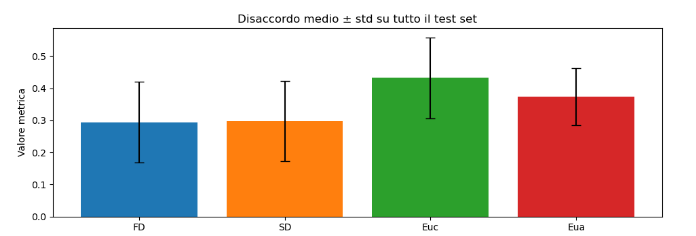
\includegraphics[width=0.8\textwidth]{globali.png}
  \caption{Bar-plot delle metriche di disaccordo medie $\pm$ std sul test set.}
  \label{fig:global_vs_case}
\end{figure}

Il bar‐plot sintetizza le quattro metriche di disaccordo su tutto il test set:
\begin{itemize}
  \item \textbf{Feature Disagreement (FD)}: con media $\approx0.29$ e deviazione standard $\approx0.13$, indica che in media il 71\% delle top‐8 feature è condiviso tra i due modelli, con alcuni casi in cui il disaccordo supera il 40\%.
  \item \textbf{Sign Disagreement (SD)}: media $\approx0.30$, segnala che non solo cambiano le feature selezionate, ma in quasi un terzo dei casi si inverte anche il segno dell’attribuzione, ossia il “verso” dell’influenza.
  \item \textbf{Euclidean}: distanza L$_2$ media $\approx0.43$, con std $\approx0.13$, mostra una divergenza complessiva moderata nei vettori normalizzati di attributi.
  \item \textbf{Euclidean‐abs}: media $\approx0.37$, dimostra che buona parte della differenza è dovuta all’intensità delle importanze, ma che il segno amplifica ulteriormente il disaccordo complessivo.
\end{itemize}

Questa sintesi conferma che, sebbene i due modelli abbiano prestazioni quasi identiche sul test set, le spiegazioni feature‐attribution possono variare in modo consistente.


\section*{5. Case study su campione 0}
Nella seconda parte della figura~\ref{fig:global_vs_case}, vengono mostrate le explanation per il campione 0. I valori delle metriche per questo singolo esempio sono:
\[
\text{FD}_0 = 0.25,\quad
\text{SD}_0 = 0.25,\quad
\text{Euc}_0 = 0.39,\quad
\text{Eua}_0 = 0.39.
\]

\begin{figure}[htbp]
  \centering
  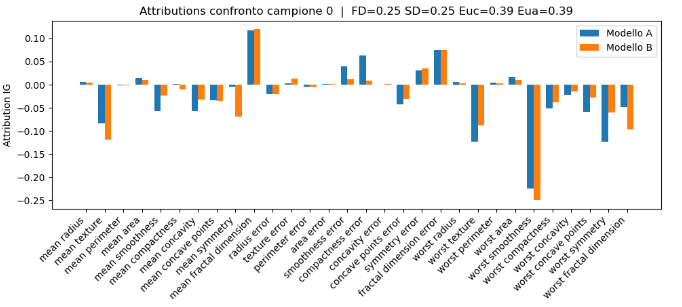
\includegraphics[width=0.8\textwidth]{campione zero.png}
  \caption{Confronto delle attribuzioni IG per il campione 0.}
  \label{fig:global_vs_case}
\end{figure}

\subsection*{Cosa mostrano le barre}
Ogni coppia di barre (blu + arancio) corrisponde a una feature del dataset Breast–Cancer (sull’asse orizzontale). 
L’altezza di ciascuna barra è il valore di attribuzione:
\begin{itemize}
  \item positivo $\to$ feature che "spinge" la rete verso la classe positiva (maligno);
  \item negativo $\to$ feature che "spinge" verso la classe negativa (benigno).
\end{itemize}
Confrontando Modello A vs. Modello B si evidenzia dove e quanto i due modelli differiscono nell'attribuire importanza.

\end{document}
